\begin{figure*}[t]
\centering
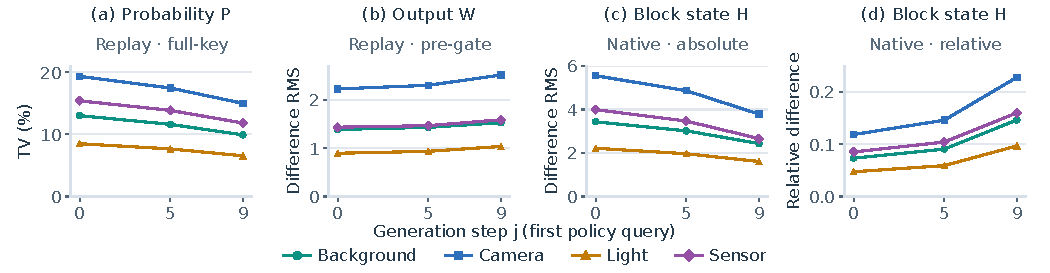
\includegraphics[width=\textwidth]{revised_figures/figure5_attention.pdf}
\caption{\textbf{Attention-weight differences shrink while output-feature differences grow.} At L18, (a) full-key probability TV decreases from the first to the last sampled generation step, while (b) the raw RMS difference in the projected attention output increases. Both are recomputed at each run's saved generation states. The block-end state recorded during the policy's own generation has (c) decreasing absolute differences but (d) increasing differences relative to the shrinking clean state. All panels use the same 404 $\pi_{0.5}$ pairs on 28 tasks; points show task-equal means for each perturbation family at steps 0, 5, and 9, without intervals. Relative responses are formed per case before averaging. Complete profiles and recording scope: Secs.~\ref{sec:supp-plus-joint-readout}, \ref{sec:plus-sites}, \ref{sec:supp-protocol-validation}, and~\ref{sec:supp-attention-views}.}
\label{fig:attention-trends}
\end{figure*}
